\documentclass[12pt]{article}
\usepackage{subcaption}
\usepackage[margin=1in]{geometry} 
\usepackage{amsmath,amsthm,amssymb}
\usepackage[english]{babel}
\usepackage{float}
\usepackage{graphicx}
\usepackage{enumitem}
\usepackage{amsmath}
\usepackage{minted}

\newcommand*{\vcenteredhbox}[1]{\begingroup
\setbox0=\hbox{#1}\parbox{\wd0}{\box0}\endgroup}
 
\begin{document}
 
% --------------------------------------------------------------
%                         BODY
% --------------------------------------------------------------
 
\title{Peer to Peer Systems and Blockchains \\ mid-term assignment}
\author{Giacomo De Liberali \\ Analyzing the Kademlia DHT}

\maketitle

\tableofcontents

\section{Introduction}

The goal of this project is to simulate the construction of a peer to peer network managed under a simplified implementation of Kademlia protocol. The simulation consists in joining a set of nodes and analyze how their routing table are populated, according to the parameters that Kademlia proposes. The simulation is developed in .NET Core C\#, the cross platform version of the Microsoft's popular framework, while network analysis is performed in Python. 



\subsection{Architecture}

\begin{figure}[H]
    \centering
    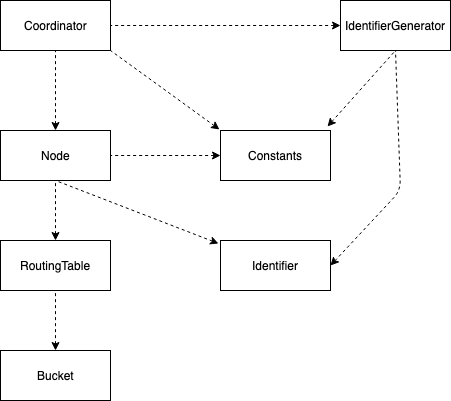
\includegraphics[width=0.6\textwidth]{assets/architecture.png}
    \caption{Code architecture}
    \label{fig:code_architecture}
\end{figure}
The \textit{Coordinator} is the entity who manages the list of joined nodes and handles the bootstrap phase of the network. It has a strict dependency on: \textit{Node}, \textit{Constants}, \textit{IdentifierGenerator}. The \textit{IdentifierGenerator} keeps track of the existing identifiers (to avoid collisions) and exposes some utility methods  sfor generating random identifiers within a specified range. \textit{Constants} is a wrapper class around available parameters, like:
\begin{itemize}
    \item $n$: the number of nodes that will join the network
    \item $m$: the number of bits used to represent the identifiers space
    \item $k$: the number of entries a bucket can contain
    \item $\alpha$: the number of \textit{findNode()} that the \textit{lookup()} procedure will subsequently call
\end{itemize}
The \textit{Node} class instead, has a dependency on the \textit{Identifier} implementation and on the \textit{Constants}, which is accessed as a static property of the central \textit{Coordinator}. The \textit{Node} class contains the implementation of the \textit{findNode()} and \textit{lookup()} procedures, as well as a reference to its own routing table. The \textit{RoutingTable} class contains a list of \textit{Buckets} and a method to access to the correct bucket when inserting a new element in the routing table. It also provide a method to return the $k$ known nodes closest to the specified target node. For "closeness" we mean the lowest \textit{XOR} distance between identifiers, as described in Kademlia's specs.

\subsection{Identifiers}

Identifiers have their own class, but internally they are represented as \textit{BigInt}, a built-in class used to express arbitrarily large signed integers. In this assignment I chose not to use hashing functions (eg. \textit{SHA3}) since their properties, such as collision resistance, were not exploited provided that those functions were applied on random generated integers.
As consequence, identifiers space ranges between $0$ and $2^m - 1$.

\section{Kademlia procedures}

The following section contains the descriptions of the main Kademlia procedures implemented in this assignment, \textit{findNode()} and \textit{lookup()}.

\subsection{FindNode}
The signature of the \textit{findNode()} is the following:
\begin{minted}{csharp}
    public FindNodeResponse FindNode(Identifier target, List<Node> traveledNodes)
\end{minted}
It takes as parameters the identifier of the target node that is has to look for and the list of the nodes that have been traversed. This procedure add to the routing table of the node on which is invoked all the nodes inside the \textit{traveledNodes} list, add itself to that list and return the updated list together with the list of the closest known nodes to the target, without any further call. This procedure is exploited iteratively by the \textit{lookup()}.

\subsection{Lookup}

The \textit{lookup()} is the core of Kademlia protocol: it populates the routing table of all the nodes, calling the \textit{findNode()} procedure several times. The \textit{Coordinator} once added the first bootstrap node to the network, generates a new node, select a joined node as its bootstrap and finally generate an identifier for each new-node's bucket. For each of these identifier it ask the new node to perform a \textit{lookup()} of that identifier, in order to make the population of the routing tables begin. \\

\noindent
My implementation of this procedure has the following pseudo-code:

\begin{minted}{csharp}
    public List<Node> Lookup(Identifier target)
    {
        // make an initial findNode
        var findNodeResponse = FindNode(target)
        // sort and take first alpha
        var alphaNotQueriedNodes = findNodeResponse.CloesetNodes
        // save traveledNodes
        var traveledNodes = findNodeResponse.TraveledNodes
        // initialize return value
        var kAbsoluteClosest = new List<Node>()
        do
        {
            foreach(node in alphaNotQueriedNodes)
            {
                var response = node.FindNode(target, traveledNodes)
                currentNodes = merge(currentNodes, response.ClosestNodes)
            }
            
            // insert nodes in k-buckets
            UpdateRoutingTable(currentNodes)
            
            // sort and take best k from merge
            kAbsoluteClosest = kAbsoluteClosest
                        .Concat(currentNodes) // concatenate with actual run
                        .Distinct() // remove duplicates
                        .OrderBy(distance to target) // asc
                        .Take(k)
            
            alphaNotQueriedNodes = kAbsoluteClosest
                        .Where(not queried)
                        .Take(alpha)
            
        }while(more closer nodes are returned)
        
        foreach(notQueriedNode in kAbsoluteClosest)
        {
            // further enrich routing tables
            node.FindNode(target, traveledNodes)
        }
        
        return kAbsoluteClosest
    }
\end{minted}

\pagebreak

\section{Network graph analysis}

The simulator takes as command line parameters the values for $n$, $m$, $k$, then generates a \textit{CSV} file containing the edges table of the resulting graph. A bash script will launch the simulator with different parameters to generate several simulations:
\begin{minted}{bash}
    for k in 1 5 20
        for n in 100 200 300 400 500 600 700 800 900 1000
            for m in 9 10 64 160
                for i in 1 2 3 # make 3 simulation with same params
                    ./kademlia.sh $n $m $k
\end{minted}
\noindent
After the generation of all the networks, a Python script will parse their graphs, analyze them with \textit{NetworkX} and create a report with average values for each triplet of parameters. The report is used to produce next plots, exploting \textit{matplotlib}, a plotting framework. 

The values of the network are relatively small because of performance issues of the \textit{NetworkX} library, in which also core algorithms are entirely written in Python.

\subsection{Network topology example}

Here we can easily notice how the parameter $k$, which indicates the capacity of each bucket, is the major player in influencing network topology. A value of $k=1$ means that each node has at most $m$ buckets each containing only a single link, and thus it has low resiliency to node failures and a higher average path length, crucial features of this kinds of P2P networks.

\begin{figure}[H]
    \centering
    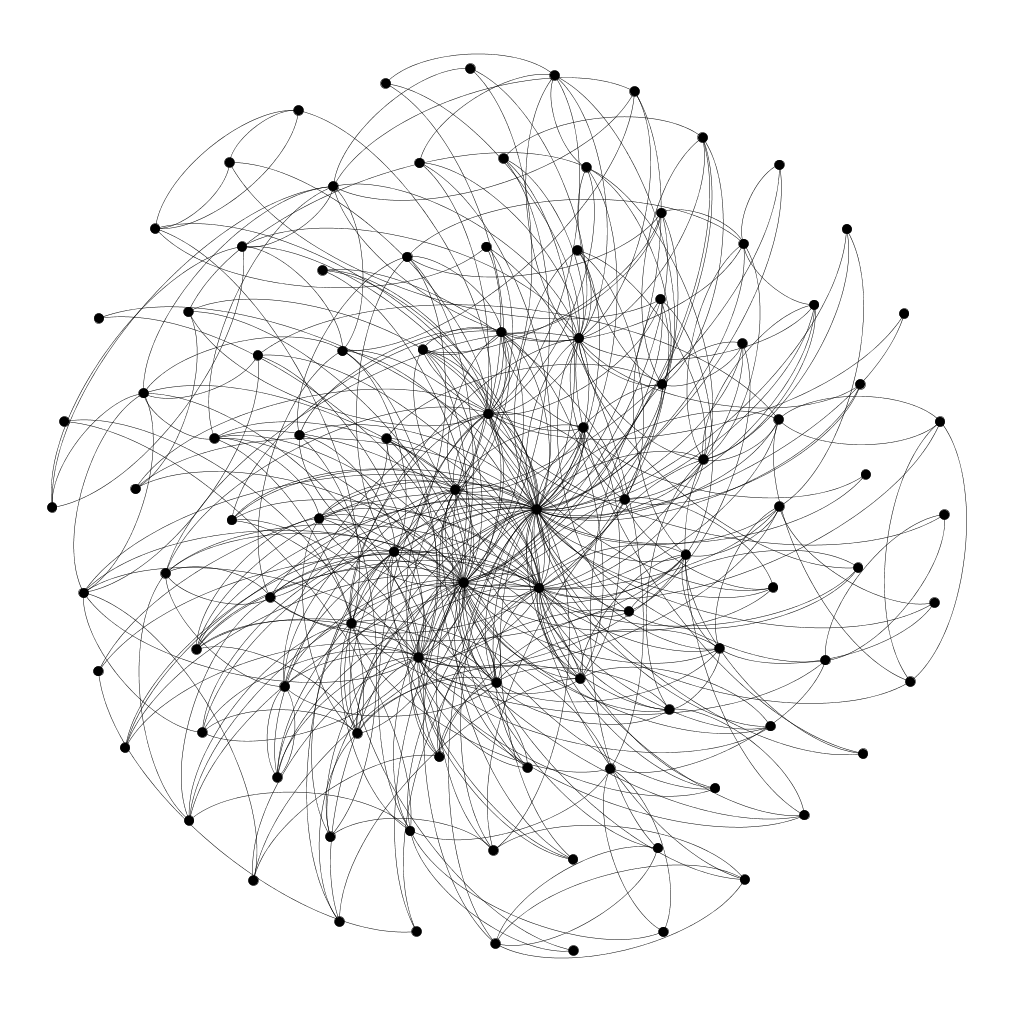
\includegraphics[width=0.3\textwidth]{assets/k1.png}
    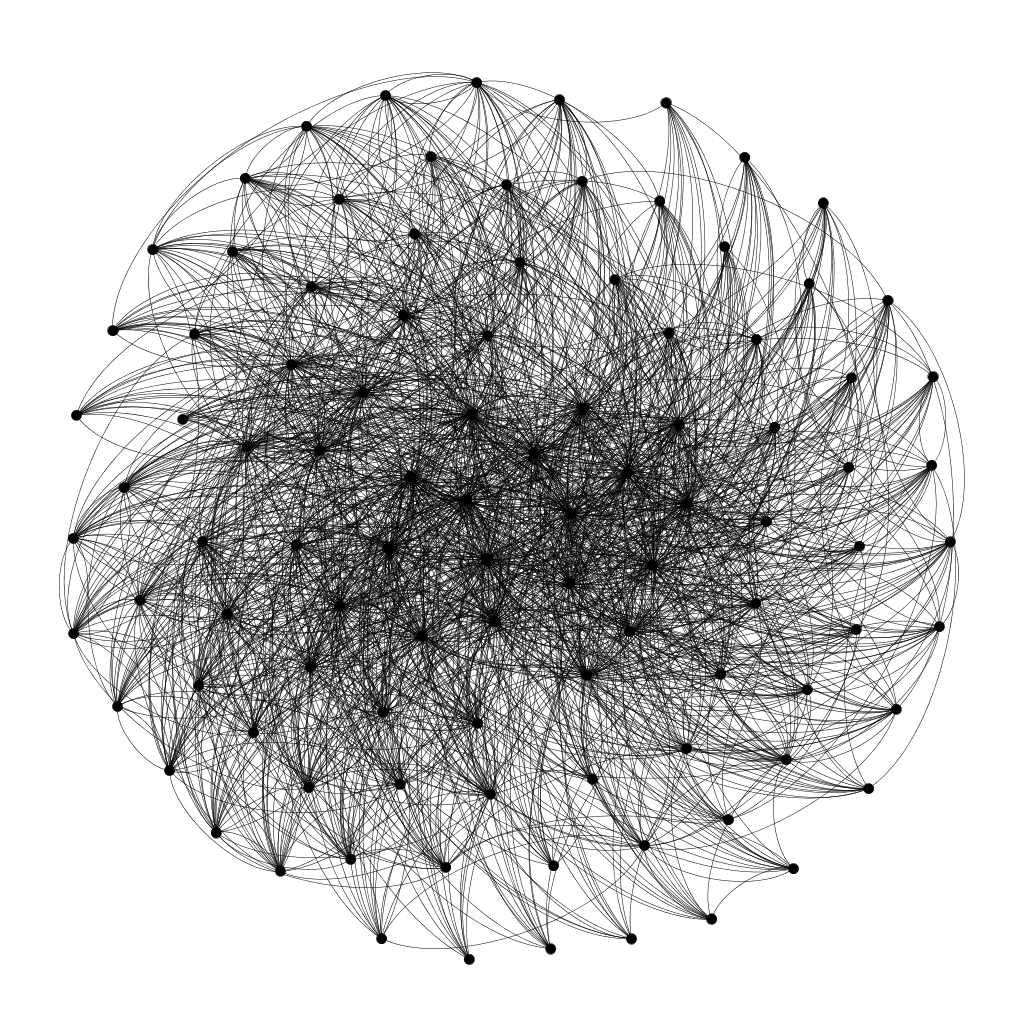
\includegraphics[width=0.3\textwidth]{assets/k5.png} 
    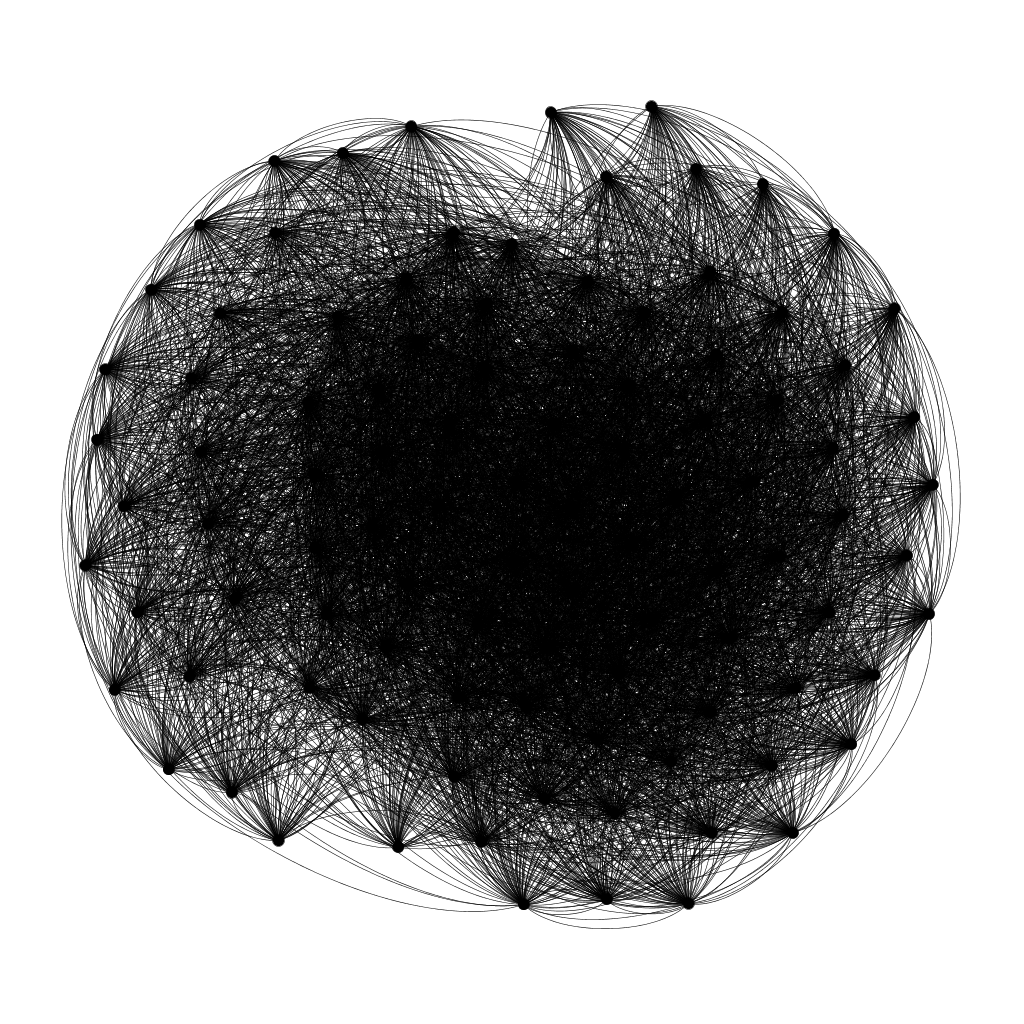
\includegraphics[width=0.3\textwidth]{assets/k20.png}
    \caption{Network with n=100, m=10, k=1, 5, 20}
    \label{fig:graph_n10_m160_k1520_alpha3}
\end{figure}

\pagebreak

\subsection{Average degree}

In the figure \ref{fig:avg_degree} we can notice the value of $k$ has a huge impact on the degree level: this is as expected since incrementing $k$ we are increasing the number of links a node can store. 

\noindent
The degree level is very important since more links a node can hold, less time a \textit{findNode()} will require since the average path length would be smaller.

\begin{figure}[H]
    \centering
    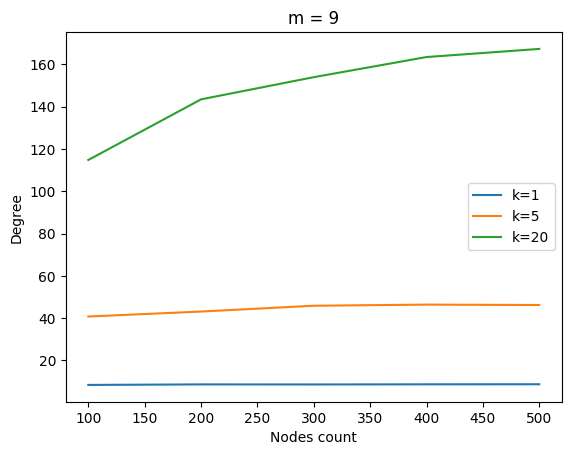
\includegraphics[width=0.45\textwidth]{assets/avg_degree_m9.png} 
    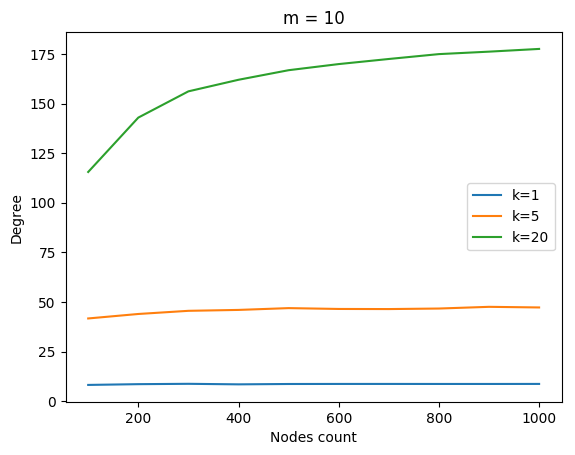
\includegraphics[width=0.45\textwidth]{assets/avg_degree_m10.png} 
    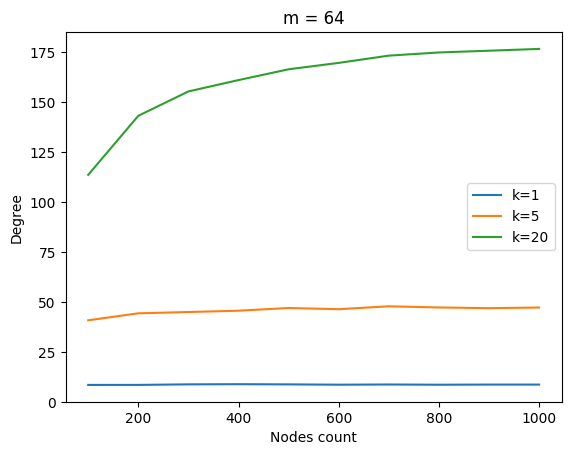
\includegraphics[width=0.45\textwidth]{assets/avg_degree_m64.png}
    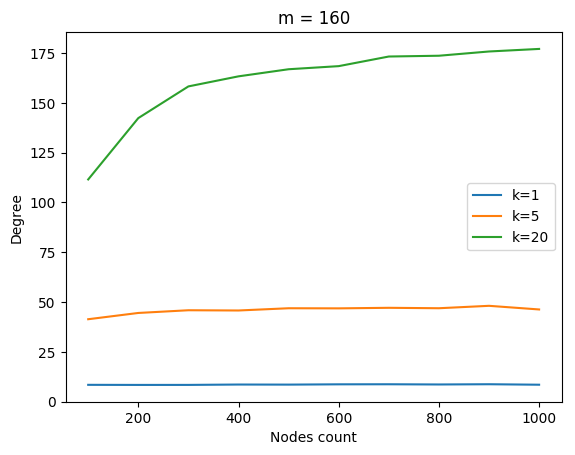
\includegraphics[width=0.45\textwidth]{assets/avg_degree_m160.png} 
    \caption{Average degree for different values of $k$ and $m$}
    \label{fig:avg_degree}
\end{figure}

\noindent
The parameter $m$ seems not to influence the average degree, as shown in figure \ref{fig:avg_degree}, where the same trend is obtained with different values of $m$, even when the number of nodes is close to the cardinality of identifiers space (eg. with $m=10$ and $n=1000$). 

\pagebreak

\subsection{Average path length}

The path length is a critic feature of this kind of networks, where nodes have to spread queries over the network in order to find the desired content. We can notice how the path length slightly grows with respect to the number of nodes, and also that an increase of $k$ brings an improvement in shorten the path length, as shown in figure \ref{fig:avg_pathlength}. 

\begin{figure}[H]
    \centering
    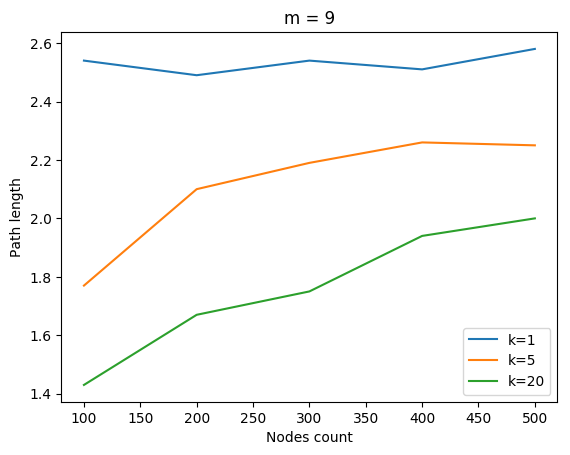
\includegraphics[width=0.45\textwidth]{assets/pathlength_m9.png}
    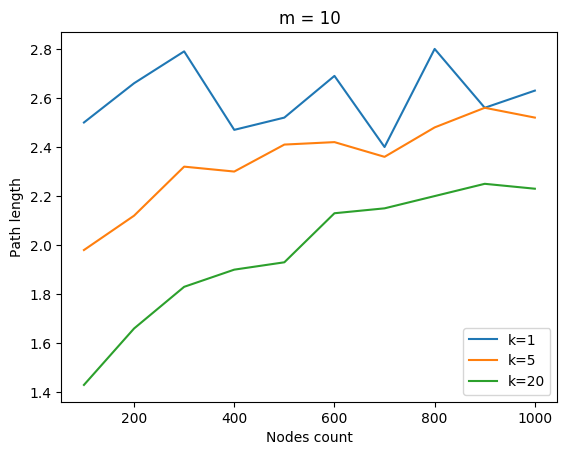
\includegraphics[width=0.45\textwidth]{assets/pathlength_m10.png}
    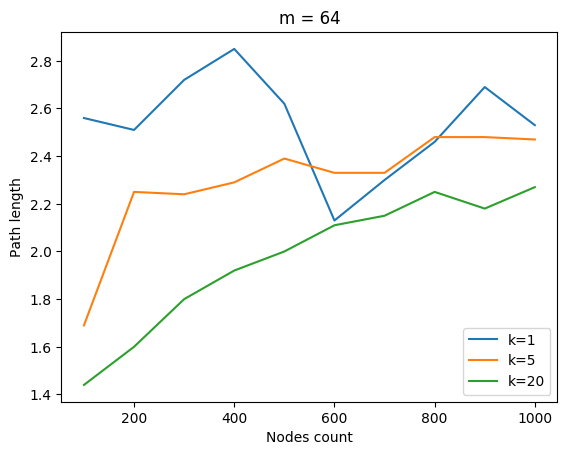
\includegraphics[width=0.45\textwidth]{assets/pathlength_m64.png}
    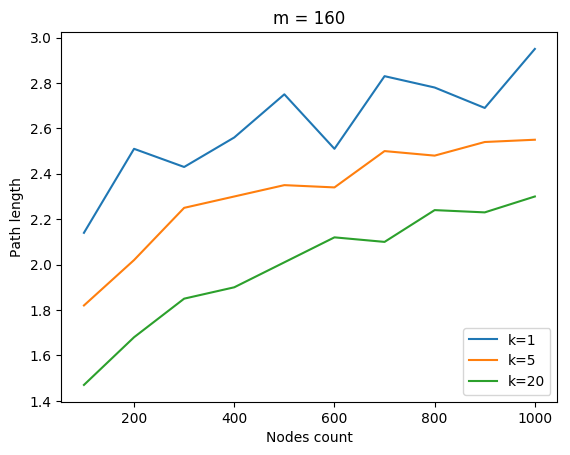
\includegraphics[width=0.45\textwidth]{assets/pathlength_m160.png}
    \caption{Average path length for different values of $k$ and $m$}
    \label{fig:avg_pathlength}
\end{figure}

\noindent
This average path reduction inducted by increasing $k$ is due to the fact that higher values of $k$ allow a node to know more
nodes, hence the number of hops needed to reach another node is smaller. \\

\pagebreak

\noindent
In this section are missing plots regarding the network diameter; the \textit{networkx.diameter(Graph)} library function is currently raising an exception that didn't allow me to compute stats on this parameter. Manual test that I've created on larger networks are summarized in figure \ref{fig:avg_diameter}, which states that the network diameter ranges between $1$ and $6$ in networks of size $10$-$10000$ (network sizes: $10,100,250,1000,2000,5000,10000$). 

\begin{figure}[H]
    \centering
    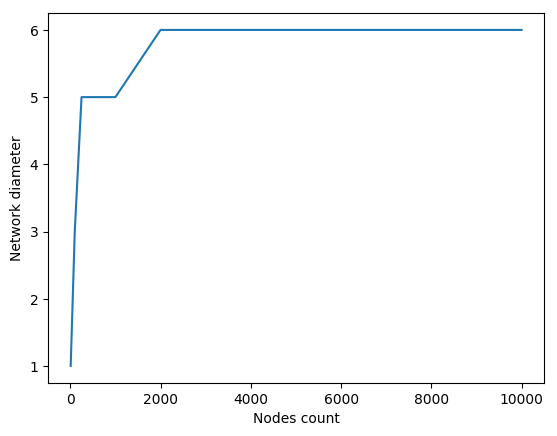
\includegraphics[width=0.45\textwidth]{assets/diameter_m160_k20.png} 
    \caption{Network diameter with m=160, k=20}
    \label{fig:avg_diameter}
\end{figure}

Network diameter remains almost constant in the last $4$ networks.


\pagebreak

\subsection{Clustering coefficient}

From figure \ref{fig:avg_clustering} we can notice that an higher value of $k$ implies a greater clustering coefficient because of the bucket's size growth and the increased number of nodes in the routing tables.
Considering $n$, we can see that if $n$ increases the clustering coefficient seems to decrease. This is as expected, since more nodes are present, more edges are needed to preserve the \textit{CC}.

\begin{figure}[H]
    \centering
    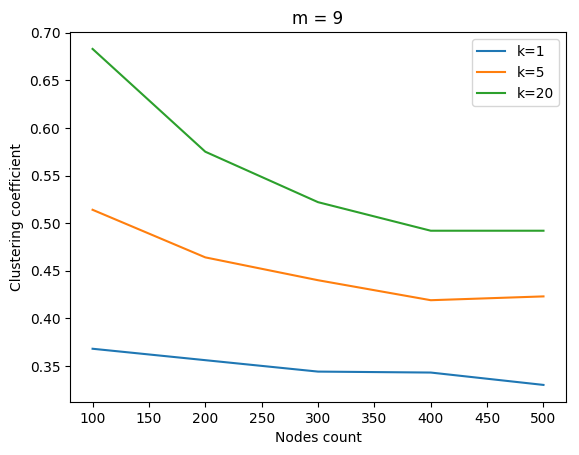
\includegraphics[width=0.45\textwidth]{assets/avg_clustering_m9.png} 
    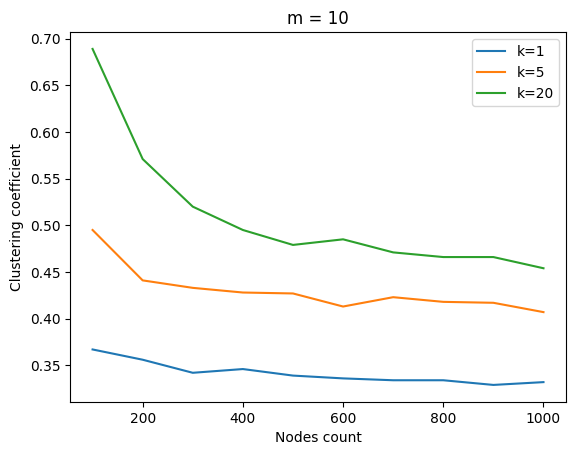
\includegraphics[width=0.45\textwidth]{assets/avg_clustering_m10.png} 
    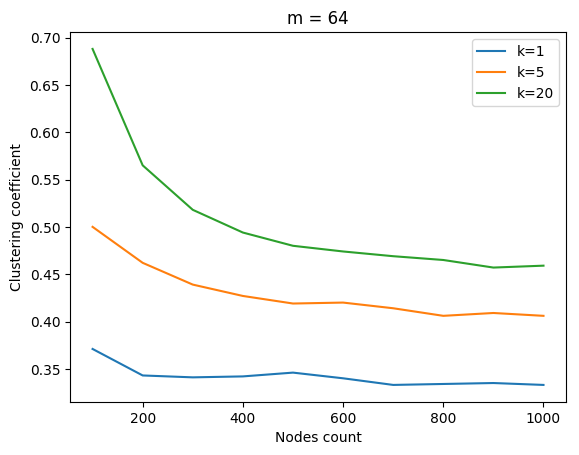
\includegraphics[width=0.45\textwidth]{assets/avg_clustering_m64.png}
    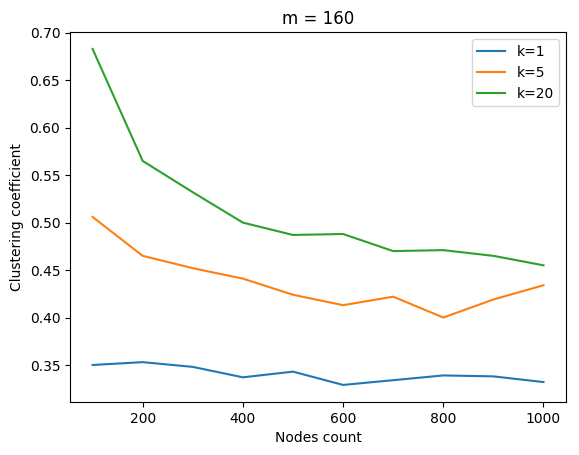
\includegraphics[width=0.45\textwidth]{assets/avg_clustering_m160.png}
    \caption{Clustering coefficient for different values of $k$ and $m$}
    \label{fig:avg_clustering}
\end{figure}

\pagebreak

\subsection{Bigger networks}

Due to performance issues of \textit{NetworkX} I've created only a single simulation on a lager network and I have analyzed it through \textit{Cytoscape}.

\begin{table}[H]
\centering
\begin{tabular}{|l|c|}
n                      & 10000 \\
m                      & 160   \\
k                      & 20    \\
diameter               & 6     \\
avg path length        & 3.046 \\
clustering coefficient & 0.420
\end{tabular}
\caption{Network simple parameters}
\label{table:network_params}
\end{table}


\begin{figure}[H]
    \centering
    \begin{subfigure}[t]{.7\linewidth}
        \centering
        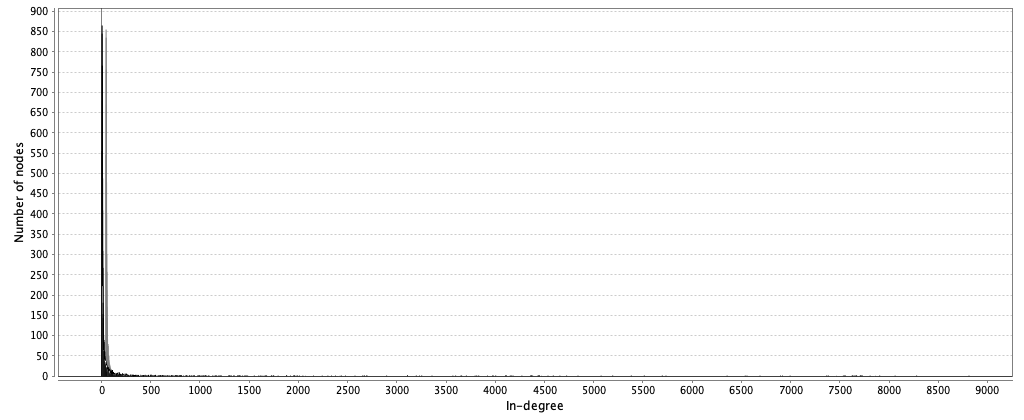
\includegraphics[width=\textwidth]{assets/in_deg_dist_n10000_m160_k20.png} 
        \caption{In-degree}
    \end{subfigure}
    
    \begin{subfigure}[t]{.7\linewidth}
        \centering
        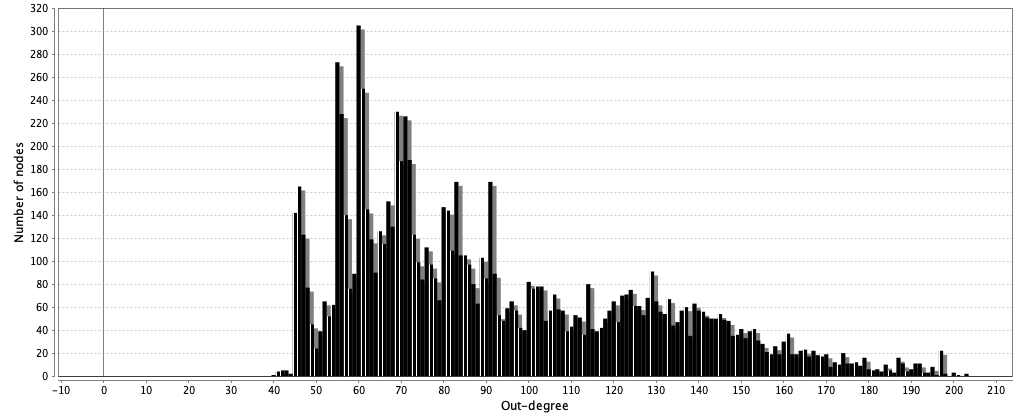
\includegraphics[width=\textwidth]{assets/out_deg_dist_n10000_m160_k20.png} 
        \caption{Out-degree}
    \end{subfigure}
    
    \caption{Degree distribution with $n=10000$, $m=160$, $k=20$}
    \label{fig:bignetwork1}
\end{figure}

\noindent
In figure \ref{fig:bignetwork1}a we can notice that the majority of network's nodes has a low in-degree value and only few of them present an high value. Nodes that show an higher value of in-degree are the ones that, with high probability, have been chosen as bootstrap from many other nodes, hence they must have joined the network at the very beginning.

\begin{figure}[H]
    \centering
    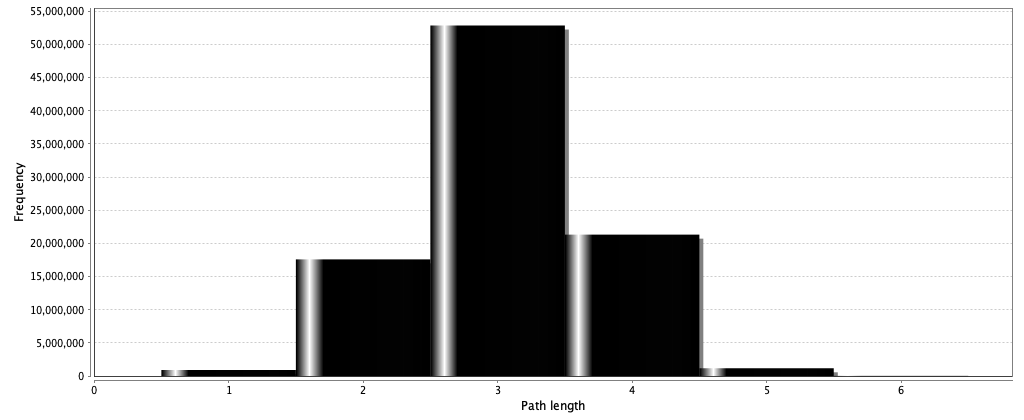
\includegraphics[width=0.7\textwidth]{assets/avg_pathlength_n10000_m160_k20.png}
    \caption{Average path length with $n=10000$, $m=160$, $k=20$}
    \label{fig:bignetwork_pathlength}
\end{figure}

\noindent
Despite the increasing number of nodes in the network, the average path length remained quite low, result that enforces the slow-growth trend highlighted in figure \ref{fig:avg_pathlength}.

\begin{figure}[H]
    \centering
    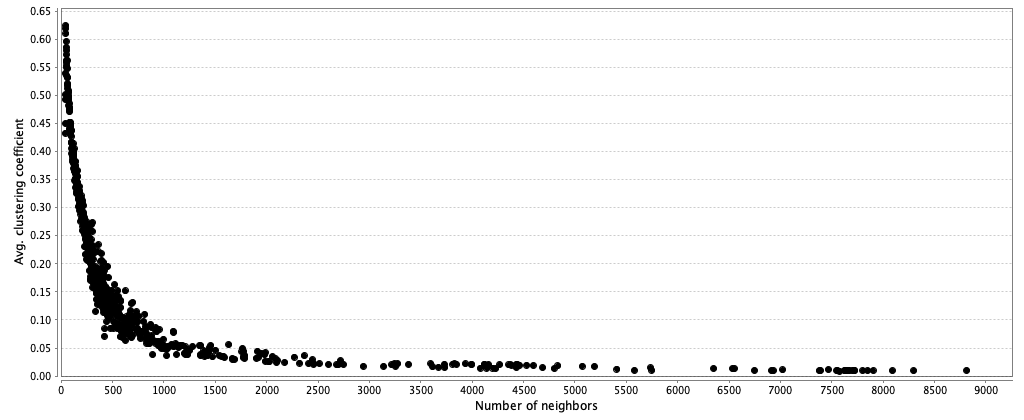
\includegraphics[width=0.7\textwidth]{assets/cc_n10000_m160_k20.png}
    \caption{Clustering coefficient with $n=10000$, $m=160$, $k=20$}
    \label{fig:bignetwork_cc}
\end{figure}

\noindent
In figure \ref{fig:bignetwork_cc} we can notice how the number of nodes ($n$) influences the clustering coefficient, highlighting results shown in figure \ref{fig:avg_clustering}.

\pagebreak

\section{Conclusions}

One goal of this assignment, beyond comparing networks properties, was automatizing as much as possible the computation of stats, allowing to quickly make experiments varying parameters. One issues raised in this scenario was the choice of the network analysis tool. One of the suggested framework was \textit{NetworkX}, but it has a huge drawback: it offers simplicity of use instead of performance. This brought me to simulate only small networks (analysis of a single network of $n=10000$, $m=160$ and $k=20$ was manual aborted after 6 hours). 

One possible future fix would be to change the graph analysis tool in order to perform simulations with higher values of $n$, allowing to better estimate trends described in this report. Another improvement to this solution would involve parallelizing the code or launching this program on a more performant machine. \\

\noindent
Despite this technical issue, analysis of networks typologies have shown that the crucial parameter in shaping Kademlia network seems to be $k$. Choosing values of $k$ around 20 can bring to good trade offs between degree, path length, diameter and clustering coefficient. 

 
% --------------------------------------------------------------
%                       END BODY
% --------------------------------------------------------------
 
\end{document}
